\documentclass[a4paper, 12pt, titlepage]{article}
\usepackage{listings,amssymb, amsmath, amsthm, graphicx, float}
\author{Joris Stork: 6185320 \and Lucas Swartsenburg: 6174388 \and Sander van
Veen: 6167969}
\title{Laboratory log book Robotics}
\begin{document}
\maketitle

\section{I$^2$C and the CSS Compiler} % {{{

\subsection{Objective} % {{{

Our objective is to implement an I$^2$C bus using: a 3-state word generator, an
I/O expander and a microcontroller (these are described below). 
The I$^2$C bus is a two-wire serial bus used for data transport between
integrated circuits.

% }}}

\subsection{Method} % {{{
Our implementation of the I$^2$C bus involves transporting 8 parallel bits of data -
generated by a human operator via the interface of a word generator -
over from the I/O expander using the 2 bit I$^2$C protocol to the microcontroller, and
back again. We programmed the
microcontroller in a C-like language and used the provided C API (functions
\texttt{i2c\_read} and \texttt{i2c\_write}) to act as the master on the I$^2$C
bus, with the I/O expander as slave (see the appendix for code). 
We connected the microcontroller's C4 and C3 pins with the I/O expander's
SDA (serial data line) and SCL (serial clock line) pins respectively. The I/O
expander's eight left-hand side pins were connected to the corresponding eight
pins of the word generator.
The program loaded onto the microcontroller initiates the transfer on the bus,
first setting the SDA signal to ``low'', then  
indicating the transmission direction (from slave to master) and the address of
the slave (corresponding to the left-hand pins of the I/O expander) from which
to send the data. Once the microcontroller had received the data, the program
initiated a second transfer in the opposite direction, sending the same data it
had received back to the I/O expander for display on the I/O expander's
right-hand LEDs.

% }}}

\subsubsection{Hardware}

\begin{itemize}
\item PCF8574 I$^2$C I/O expander integrated circuit (IC).
Each of this I/O expander's eight pins can be used as an input or output. In order 
to use a pin as input, a 1 has to be written to that pin's register.
\item 16F876 microcontroller: this is an 8 bit microcontroller that we load with
programs written in mplab \dots
\item 74LS244 word (8 bit) generator. Buttons toggle each of the eight pins
representing the 8 bits of output.
\end{itemize}

\subsubsection{Software}
The follows software runs on an i86 Windows XP machine which is connected to the
microcontroller using a serial port cable.
\begin{itemize}
\item Tera Term Web 3.1 : used as a terminal console for the microcontroller.
\item MPLAB IDE v6.30
\item PIDAC 876 programmer: Loads the compiled program onto the microcontroller
using the serial port.
\end{itemize}

% }}}

% }}}

\subsection{results} % {{{
The experiment worked as expected. The \texttt{0b11000110} was transmitted and
returned successfully, as shown in the image below:
\begin{figure}[H]
\caption{The set-up}
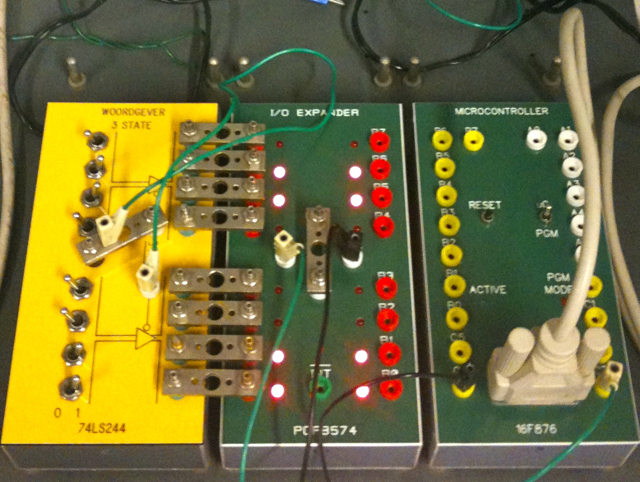
\includegraphics[scale=0.61]{IMG_0703}
\end{figure}
% }}}

\subsection{assumptions} % {{{

% }}}

\section{sar adc} % {{{

\subsection{objective} % {{{

% }}}

\subsection{method} % {{{

% }}}

\subsection{equipment} % {{{

% }}}

\subsection{raw results} % {{{

% }}}

\subsection{results} % {{{

% }}}

\subsection{assumptions} % {{{

% }}}

% }}}

\section{servo system} % {{{

\subsection{objective} % {{{

% }}}

\subsection{method} % {{{

% }}}

\subsection{equipment} % {{{

% }}}

\subsection{raw results} % {{{

% }}}

\subsection{results} % {{{

% }}}

\subsection{assumptions} % {{{

% }}}

% }}}

\newpage
\appendix

\section{Source: i$^2$c} % {{{
\begin{verbatim}
/////////////////////////////////////////////////////////////////////////
//
// Filename 	:	Test876.c                                            
// Revision 	:	1.0                                                   
// Created  	:	19-3-2001 
// Revised	: 	26-11-2003 by Benb       
                                   
// Project  	:	Pidac876                                              
// Device		:	PIC16F876                                          
// Development	:	MPLAB / CCS PCM                                                        
// Author		:	E. Steffens
// Department	:	Faculty of science
// Copyright	:	Universiteit van Amsterdam
//Description	:	Testing serial connection with PC                        
/////////////////////////////////////////////////////////////////////////

#include <C:\Program Files\PICC\Devices\16F876.H>
#include <C:\Program Files\PICC\Drivers\CTYPE.H>

// Inform the compiler the clock frequency is 8 MHz
#use delay(clock=8000000) 

// Setup the RS232 communication
#use rs232(baud=9600, xmit=PIN_C6, rcv=PIN_C7,  bits=8)

//Setup the I2C bus
#use I2C (Master, SDA=PIN_C4, SCL=PIN_C3, SLOW)

int main(){
	int Getal = 0;
    int Getal_1 = 0;
    printf("Assignment 4 \n\r");

	//Voorbeeld: Byte van Master ? Slave met adres 1

	while(1){
	//Voorbeeld: Byte van Slave met adres 0 ? Master 
	i2c_start();
	i2c_write( 0x41 );//write address (01000001)
	Getal = i2c_read(0); // acknowledge
	i2c_stop();

	i2c_start();
	i2c_write( 0x42 );//write address (01000010)
	i2c_write( Getal );	//write byte
	i2c_stop();
	if(Getal!=Getal_1){
        printf("%d \n\r", Getal);
        Getal_1 = Getal;
    }
    }
  return 0;
}
\end{verbatim}
% }}}

\section{source: sar adc} % {{{

% }}}

\section{source: servo system} % {{{

% }}}

\end{document}
